% Created by tikzDevice version 0.12 on 2019-07-24 04:41:27
% !TEX encoding = UTF-8 Unicode
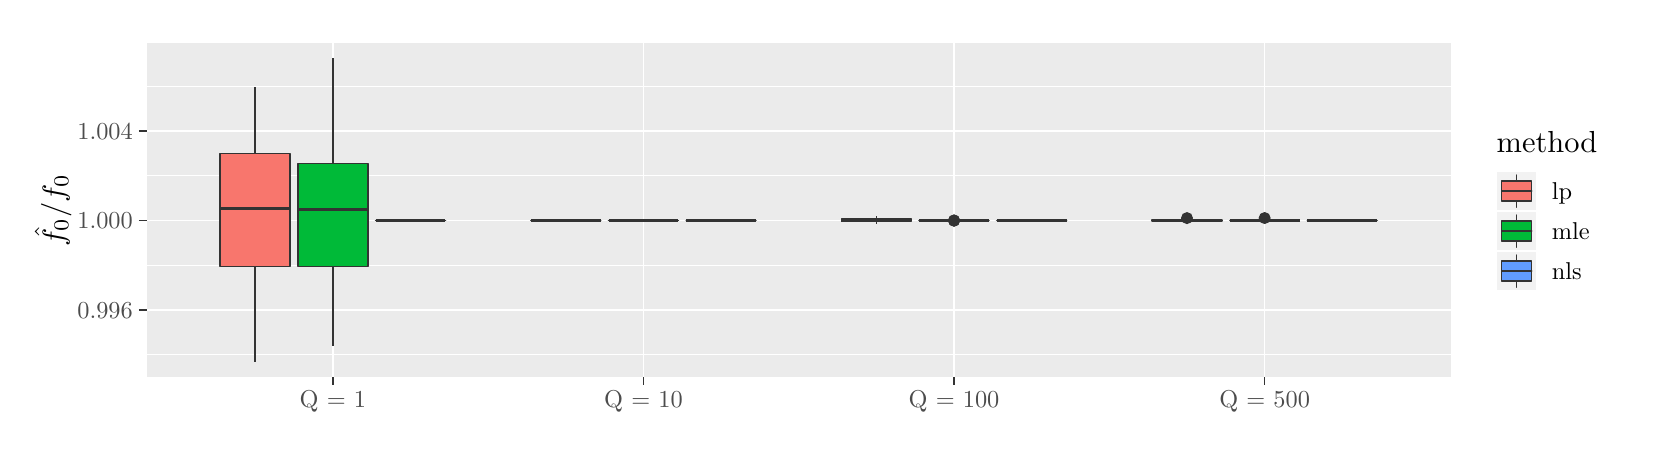
\begin{tikzpicture}[x=1pt,y=1pt]
\definecolor{fillColor}{RGB}{255,255,255}
\path[use as bounding box,fill=fillColor,fill opacity=0.00] (0,0) rectangle (578.16,144.54);
\begin{scope}
\path[clip] (  0.00,  0.00) rectangle (578.16,144.54);
\definecolor{drawColor}{RGB}{255,255,255}
\definecolor{fillColor}{RGB}{255,255,255}

\path[draw=drawColor,line width= 0.6pt,line join=round,line cap=round,fill=fillColor] (  0.00,  0.00) rectangle (578.16,144.54);
\end{scope}
\begin{scope}
\path[clip] ( 42.95, 18.22) rectangle (514.31,139.04);
\definecolor{fillColor}{gray}{0.92}

\path[fill=fillColor] ( 42.95, 18.22) rectangle (514.31,139.04);
\definecolor{drawColor}{RGB}{255,255,255}

\path[draw=drawColor,line width= 0.3pt,line join=round] ( 42.95, 26.39) --
	(514.31, 26.39);

\path[draw=drawColor,line width= 0.3pt,line join=round] ( 42.95, 58.69) --
	(514.31, 58.69);

\path[draw=drawColor,line width= 0.3pt,line join=round] ( 42.95, 90.99) --
	(514.31, 90.99);

\path[draw=drawColor,line width= 0.3pt,line join=round] ( 42.95,123.29) --
	(514.31,123.29);

\path[draw=drawColor,line width= 0.6pt,line join=round] ( 42.95, 42.54) --
	(514.31, 42.54);

\path[draw=drawColor,line width= 0.6pt,line join=round] ( 42.95, 74.84) --
	(514.31, 74.84);

\path[draw=drawColor,line width= 0.6pt,line join=round] ( 42.95,107.14) --
	(514.31,107.14);

\path[draw=drawColor,line width= 0.6pt,line join=round] (110.29, 18.22) --
	(110.29,139.04);

\path[draw=drawColor,line width= 0.6pt,line join=round] (222.52, 18.22) --
	(222.52,139.04);

\path[draw=drawColor,line width= 0.6pt,line join=round] (334.74, 18.22) --
	(334.74,139.04);

\path[draw=drawColor,line width= 0.6pt,line join=round] (446.97, 18.22) --
	(446.97,139.04);
\definecolor{drawColor}{gray}{0.20}

\path[draw=drawColor,line width= 0.6pt,line join=round] ( 82.23, 99.04) -- ( 82.23,123.08);

\path[draw=drawColor,line width= 0.6pt,line join=round] ( 82.23, 58.28) -- ( 82.23, 23.71);
\definecolor{fillColor}{RGB}{248,118,109}

\path[draw=drawColor,line width= 0.6pt,line join=round,line cap=round,fill=fillColor] ( 69.61, 99.04) --
	( 69.61, 58.28) --
	( 94.86, 58.28) --
	( 94.86, 99.04) --
	( 69.61, 99.04) --
	cycle;

\path[draw=drawColor,line width= 1.1pt,line join=round] ( 69.61, 79.33) -- ( 94.86, 79.33);

\path[draw=drawColor,line width= 0.6pt,line join=round] (110.29, 95.43) -- (110.29,133.55);

\path[draw=drawColor,line width= 0.6pt,line join=round] (110.29, 58.26) -- (110.29, 29.61);
\definecolor{fillColor}{RGB}{0,186,56}

\path[draw=drawColor,line width= 0.6pt,line join=round,line cap=round,fill=fillColor] ( 97.66, 95.43) --
	( 97.66, 58.26) --
	(122.92, 58.26) --
	(122.92, 95.43) --
	( 97.66, 95.43) --
	cycle;

\path[draw=drawColor,line width= 1.1pt,line join=round] ( 97.66, 78.86) -- (122.92, 78.86);

\path[draw=drawColor,line width= 0.6pt,line join=round] (138.35, 74.84) -- (138.35, 74.84);

\path[draw=drawColor,line width= 0.6pt,line join=round] (138.35, 74.84) -- (138.35, 74.84);
\definecolor{fillColor}{RGB}{97,156,255}

\path[draw=drawColor,line width= 0.6pt,line join=round,line cap=round,fill=fillColor] (125.72, 74.84) --
	(125.72, 74.84) --
	(150.97, 74.84) --
	(150.97, 74.84) --
	(125.72, 74.84) --
	cycle;

\path[draw=drawColor,line width= 1.1pt,line join=round] (125.72, 74.84) -- (150.97, 74.84);

\path[draw=drawColor,line width= 0.6pt,line join=round] (194.46, 74.84) -- (194.46, 74.84);

\path[draw=drawColor,line width= 0.6pt,line join=round] (194.46, 74.84) -- (194.46, 74.84);
\definecolor{fillColor}{RGB}{248,118,109}

\path[draw=drawColor,line width= 0.6pt,line join=round,line cap=round,fill=fillColor] (181.83, 74.84) --
	(181.83, 74.84) --
	(207.09, 74.84) --
	(207.09, 74.84) --
	(181.83, 74.84) --
	cycle;

\path[draw=drawColor,line width= 1.1pt,line join=round] (181.83, 74.84) -- (207.09, 74.84);

\path[draw=drawColor,line width= 0.6pt,line join=round] (222.52, 74.84) -- (222.52, 74.84);

\path[draw=drawColor,line width= 0.6pt,line join=round] (222.52, 74.84) -- (222.52, 74.84);
\definecolor{fillColor}{RGB}{0,186,56}

\path[draw=drawColor,line width= 0.6pt,line join=round,line cap=round,fill=fillColor] (209.89, 74.84) --
	(209.89, 74.84) --
	(235.14, 74.84) --
	(235.14, 74.84) --
	(209.89, 74.84) --
	cycle;

\path[draw=drawColor,line width= 1.1pt,line join=round] (209.89, 74.84) -- (235.14, 74.84);

\path[draw=drawColor,line width= 0.6pt,line join=round] (250.57, 74.84) -- (250.57, 74.84);

\path[draw=drawColor,line width= 0.6pt,line join=round] (250.57, 74.84) -- (250.57, 74.84);
\definecolor{fillColor}{RGB}{97,156,255}

\path[draw=drawColor,line width= 0.6pt,line join=round,line cap=round,fill=fillColor] (237.95, 74.84) --
	(237.95, 74.84) --
	(263.20, 74.84) --
	(263.20, 74.84) --
	(237.95, 74.84) --
	cycle;

\path[draw=drawColor,line width= 1.1pt,line join=round] (237.95, 74.84) -- (263.20, 74.84);

\path[draw=drawColor,line width= 0.6pt,line join=round] (306.69, 75.42) -- (306.69, 76.37);

\path[draw=drawColor,line width= 0.6pt,line join=round] (306.69, 74.62) -- (306.69, 73.57);
\definecolor{fillColor}{RGB}{248,118,109}

\path[draw=drawColor,line width= 0.6pt,line join=round,line cap=round,fill=fillColor] (294.06, 75.42) --
	(294.06, 74.62) --
	(319.31, 74.62) --
	(319.31, 75.42) --
	(294.06, 75.42) --
	cycle;

\path[draw=drawColor,line width= 1.1pt,line join=round] (294.06, 74.96) -- (319.31, 74.96);
\definecolor{fillColor}{gray}{0.20}

\path[draw=drawColor,line width= 0.4pt,line join=round,line cap=round,fill=fillColor] (334.74, 74.88) circle (  1.96);

\path[draw=drawColor,line width= 0.4pt,line join=round,line cap=round,fill=fillColor] (334.74, 74.81) circle (  1.96);

\path[draw=drawColor,line width= 0.4pt,line join=round,line cap=round,fill=fillColor] (334.74, 74.82) circle (  1.96);

\path[draw=drawColor,line width= 0.6pt,line join=round] (334.74, 74.86) -- (334.74, 74.87);

\path[draw=drawColor,line width= 0.6pt,line join=round] (334.74, 74.84) -- (334.74, 74.83);
\definecolor{fillColor}{RGB}{0,186,56}

\path[draw=drawColor,line width= 0.6pt,line join=round,line cap=round,fill=fillColor] (322.12, 74.86) --
	(322.12, 74.84) --
	(347.37, 74.84) --
	(347.37, 74.86) --
	(322.12, 74.86) --
	cycle;

\path[draw=drawColor,line width= 1.1pt,line join=round] (322.12, 74.84) -- (347.37, 74.84);

\path[draw=drawColor,line width= 0.6pt,line join=round] (362.80, 74.84) -- (362.80, 74.84);

\path[draw=drawColor,line width= 0.6pt,line join=round] (362.80, 74.84) -- (362.80, 74.84);
\definecolor{fillColor}{RGB}{97,156,255}

\path[draw=drawColor,line width= 0.6pt,line join=round,line cap=round,fill=fillColor] (350.18, 74.84) --
	(350.18, 74.84) --
	(375.43, 74.84) --
	(375.43, 74.84) --
	(350.18, 74.84) --
	cycle;

\path[draw=drawColor,line width= 1.1pt,line join=round] (350.18, 74.84) -- (375.43, 74.84);
\definecolor{fillColor}{gray}{0.20}

\path[draw=drawColor,line width= 0.4pt,line join=round,line cap=round,fill=fillColor] (418.91, 75.73) circle (  1.96);

\path[draw=drawColor,line width= 0.6pt,line join=round] (418.91, 75.00) -- (418.91, 75.18);

\path[draw=drawColor,line width= 0.6pt,line join=round] (418.91, 74.64) -- (418.91, 74.48);
\definecolor{fillColor}{RGB}{248,118,109}

\path[draw=drawColor,line width= 0.6pt,line join=round,line cap=round,fill=fillColor] (406.29, 75.00) --
	(406.29, 74.64) --
	(431.54, 74.64) --
	(431.54, 75.00) --
	(406.29, 75.00) --
	cycle;

\path[draw=drawColor,line width= 1.1pt,line join=round] (406.29, 74.90) -- (431.54, 74.90);
\definecolor{fillColor}{gray}{0.20}

\path[draw=drawColor,line width= 0.4pt,line join=round,line cap=round,fill=fillColor] (446.97, 75.75) circle (  1.96);

\path[draw=drawColor,line width= 0.6pt,line join=round] (446.97, 74.88) -- (446.97, 74.91);

\path[draw=drawColor,line width= 0.6pt,line join=round] (446.97, 74.84) -- (446.97, 74.81);
\definecolor{fillColor}{RGB}{0,186,56}

\path[draw=drawColor,line width= 0.6pt,line join=round,line cap=round,fill=fillColor] (434.35, 74.88) --
	(434.35, 74.84) --
	(459.60, 74.84) --
	(459.60, 74.88) --
	(434.35, 74.88) --
	cycle;

\path[draw=drawColor,line width= 1.1pt,line join=round] (434.35, 74.86) -- (459.60, 74.86);

\path[draw=drawColor,line width= 0.6pt,line join=round] (475.03, 74.84) -- (475.03, 74.84);

\path[draw=drawColor,line width= 0.6pt,line join=round] (475.03, 74.84) -- (475.03, 74.84);
\definecolor{fillColor}{RGB}{97,156,255}

\path[draw=drawColor,line width= 0.6pt,line join=round,line cap=round,fill=fillColor] (462.40, 74.84) --
	(462.40, 74.84) --
	(487.65, 74.84) --
	(487.65, 74.84) --
	(462.40, 74.84) --
	cycle;

\path[draw=drawColor,line width= 1.1pt,line join=round] (462.40, 74.84) -- (487.65, 74.84);
\end{scope}
\begin{scope}
\path[clip] (  0.00,  0.00) rectangle (578.16,144.54);
\definecolor{drawColor}{gray}{0.30}

\node[text=drawColor,anchor=base east,inner sep=0pt, outer sep=0pt, scale=  0.88] at ( 38.00, 39.51) {0.996};

\node[text=drawColor,anchor=base east,inner sep=0pt, outer sep=0pt, scale=  0.88] at ( 38.00, 71.81) {1.000};

\node[text=drawColor,anchor=base east,inner sep=0pt, outer sep=0pt, scale=  0.88] at ( 38.00,104.11) {1.004};
\end{scope}
\begin{scope}
\path[clip] (  0.00,  0.00) rectangle (578.16,144.54);
\definecolor{drawColor}{gray}{0.20}

\path[draw=drawColor,line width= 0.6pt,line join=round] ( 40.20, 42.54) --
	( 42.95, 42.54);

\path[draw=drawColor,line width= 0.6pt,line join=round] ( 40.20, 74.84) --
	( 42.95, 74.84);

\path[draw=drawColor,line width= 0.6pt,line join=round] ( 40.20,107.14) --
	( 42.95,107.14);
\end{scope}
\begin{scope}
\path[clip] (  0.00,  0.00) rectangle (578.16,144.54);
\definecolor{drawColor}{gray}{0.20}

\path[draw=drawColor,line width= 0.6pt,line join=round] (110.29, 15.47) --
	(110.29, 18.22);

\path[draw=drawColor,line width= 0.6pt,line join=round] (222.52, 15.47) --
	(222.52, 18.22);

\path[draw=drawColor,line width= 0.6pt,line join=round] (334.74, 15.47) --
	(334.74, 18.22);

\path[draw=drawColor,line width= 0.6pt,line join=round] (446.97, 15.47) --
	(446.97, 18.22);
\end{scope}
\begin{scope}
\path[clip] (  0.00,  0.00) rectangle (578.16,144.54);
\definecolor{drawColor}{gray}{0.30}

\node[text=drawColor,anchor=base,inner sep=0pt, outer sep=0pt, scale=  0.88] at (110.29,  7.21) {Q = 1};

\node[text=drawColor,anchor=base,inner sep=0pt, outer sep=0pt, scale=  0.88] at (222.52,  7.21) {Q = 10};

\node[text=drawColor,anchor=base,inner sep=0pt, outer sep=0pt, scale=  0.88] at (334.74,  7.21) {Q = 100};

\node[text=drawColor,anchor=base,inner sep=0pt, outer sep=0pt, scale=  0.88] at (446.97,  7.21) {Q = 500};
\end{scope}
\begin{scope}
\path[clip] (  0.00,  0.00) rectangle (578.16,144.54);
\definecolor{drawColor}{RGB}{0,0,0}

\node[text=drawColor,rotate= 90.00,anchor=base,inner sep=0pt, outer sep=0pt, scale=  1.10] at ( 13.08, 78.63) {$\hat{f_0}/f_0$};
\end{scope}
\begin{scope}
\path[clip] (  0.00,  0.00) rectangle (578.16,144.54);
\definecolor{fillColor}{RGB}{255,255,255}

\path[fill=fillColor] (525.31, 43.84) rectangle (572.66,113.42);
\end{scope}
\begin{scope}
\path[clip] (  0.00,  0.00) rectangle (578.16,144.54);
\definecolor{drawColor}{RGB}{0,0,0}

\node[text=drawColor,anchor=base west,inner sep=0pt, outer sep=0pt, scale=  1.10] at (530.81, 99.27) {method};
\end{scope}
\begin{scope}
\path[clip] (  0.00,  0.00) rectangle (578.16,144.54);
\definecolor{drawColor}{RGB}{255,255,255}
\definecolor{fillColor}{gray}{0.95}

\path[draw=drawColor,line width= 0.6pt,line join=round,line cap=round,fill=fillColor] (530.81, 78.25) rectangle (545.26, 92.70);
\end{scope}
\begin{scope}
\path[clip] (  0.00,  0.00) rectangle (578.16,144.54);
\definecolor{drawColor}{gray}{0.20}

\path[draw=drawColor,line width= 0.6pt,line join=round,line cap=round] (538.03, 79.70) --
	(538.03, 81.86);

\path[draw=drawColor,line width= 0.6pt,line join=round,line cap=round] (538.03, 89.09) --
	(538.03, 91.26);
\definecolor{fillColor}{RGB}{248,118,109}

\path[draw=drawColor,line width= 0.6pt,line join=round,line cap=round,fill=fillColor] (532.61, 81.86) rectangle (543.45, 89.09);

\path[draw=drawColor,line width= 0.6pt,line join=round,line cap=round] (532.61, 85.48) --
	(543.45, 85.48);
\end{scope}
\begin{scope}
\path[clip] (  0.00,  0.00) rectangle (578.16,144.54);
\definecolor{drawColor}{RGB}{255,255,255}
\definecolor{fillColor}{gray}{0.95}

\path[draw=drawColor,line width= 0.6pt,line join=round,line cap=round,fill=fillColor] (530.81, 63.80) rectangle (545.26, 78.25);
\end{scope}
\begin{scope}
\path[clip] (  0.00,  0.00) rectangle (578.16,144.54);
\definecolor{drawColor}{gray}{0.20}

\path[draw=drawColor,line width= 0.6pt,line join=round,line cap=round] (538.03, 65.24) --
	(538.03, 67.41);

\path[draw=drawColor,line width= 0.6pt,line join=round,line cap=round] (538.03, 74.64) --
	(538.03, 76.81);
\definecolor{fillColor}{RGB}{0,186,56}

\path[draw=drawColor,line width= 0.6pt,line join=round,line cap=round,fill=fillColor] (532.61, 67.41) rectangle (543.45, 74.64);

\path[draw=drawColor,line width= 0.6pt,line join=round,line cap=round] (532.61, 71.02) --
	(543.45, 71.02);
\end{scope}
\begin{scope}
\path[clip] (  0.00,  0.00) rectangle (578.16,144.54);
\definecolor{drawColor}{RGB}{255,255,255}
\definecolor{fillColor}{gray}{0.95}

\path[draw=drawColor,line width= 0.6pt,line join=round,line cap=round,fill=fillColor] (530.81, 49.34) rectangle (545.26, 63.80);
\end{scope}
\begin{scope}
\path[clip] (  0.00,  0.00) rectangle (578.16,144.54);
\definecolor{drawColor}{gray}{0.20}

\path[draw=drawColor,line width= 0.6pt,line join=round,line cap=round] (538.03, 50.79) --
	(538.03, 52.96);

\path[draw=drawColor,line width= 0.6pt,line join=round,line cap=round] (538.03, 60.18) --
	(538.03, 62.35);
\definecolor{fillColor}{RGB}{97,156,255}

\path[draw=drawColor,line width= 0.6pt,line join=round,line cap=round,fill=fillColor] (532.61, 52.96) rectangle (543.45, 60.18);

\path[draw=drawColor,line width= 0.6pt,line join=round,line cap=round] (532.61, 56.57) --
	(543.45, 56.57);
\end{scope}
\begin{scope}
\path[clip] (  0.00,  0.00) rectangle (578.16,144.54);
\definecolor{drawColor}{RGB}{0,0,0}

\node[text=drawColor,anchor=base west,inner sep=0pt, outer sep=0pt, scale=  0.88] at (550.76, 82.45) {lp};
\end{scope}
\begin{scope}
\path[clip] (  0.00,  0.00) rectangle (578.16,144.54);
\definecolor{drawColor}{RGB}{0,0,0}

\node[text=drawColor,anchor=base west,inner sep=0pt, outer sep=0pt, scale=  0.88] at (550.76, 67.99) {mle};
\end{scope}
\begin{scope}
\path[clip] (  0.00,  0.00) rectangle (578.16,144.54);
\definecolor{drawColor}{RGB}{0,0,0}

\node[text=drawColor,anchor=base west,inner sep=0pt, outer sep=0pt, scale=  0.88] at (550.76, 53.54) {nls};
\end{scope}
\end{tikzpicture}
